\documentclass[french, twoside=semi, headings=normal]{scrartcl}
\usepackage{microtype}
\usepackage{babel}
\usepackage{amsmath}
\usepackage{numprint}
\usepackage{booktabs}
\usepackage[locale=FR]{siunitx}
\usepackage{pgf}
\usepackage{pgfplots}
\usepackage{unicode-math}
\usepackage{lualatex-math}
\usepackage[unicode]{hyperref}

\raggedbottom

\pgfplotsset{compat=newest}

\setmainfont{STIX Two Text}[
    Numbers = {OldStyle, Proportional},
    Scale = 0.91
]
\setmonofont{LucidaSansTypewriterOT}[
    Scale = MatchLowercase
]
\setmathfont{STIX Two Math}[
    StylisticSet = 8,
    Scale = 0.91
]
\addtokomafont{disposition}{\normalfont}
\addtokomafont{subject}{\normalfont}

\hypersetup{
    pdftitle = {Devoir 5},
    pdfsubject = {Introduction à l’apprentissage machine},
    pdfauthor = {Mathieu Alain, Julien Dethurens, Eloïse Valenti}
}

\usepackage{url}
\urldef{\mailmathieu}\path|mathieu.alain.2@ulaval.ca|
\urldef{\mailelo}\path|eloise.valenti.1@ulaval.ca|
\urldef{\mailjulien}\path|julien.dethurens.1@ulaval.ca|

\subject{Introduction à l'apprentissage machine (GIF-4101)}
\title{Devoir 5}
\author{Mathieu Alain\thanks{Département de mathématiques et de statistique --- \mailmathieu.} \and Eloise Valenti\thanks{Département d'informatique et de génie logiciel --- \mailelo.} \and Julien Dethurens\thanks{Département de mathématiques et de statistique --- \mailjulien.}}

\begin{document}

\maketitle

\section{Clustering de données}

\section{Sélection de variables}

\section{Méthodes par ensemble}

On a utilisé un classifieur par ensemble basé sur AdaBoost sur le jeu de données à quatre classes avec un maximum de \numprint{50} classifieurs de base, avec des souches de décision et avec des arbres de décision à trois niveaux.

La table~\ref{tab:adaboost_scores_with_decision_stumps} donne les performances obtenues avec des souches de décision. La performance en entraînement est dans la figure~\ref{fig:adaboost_train_scores_with_decision_stumps} et la performance en test dans la figure~\ref{fig:adaboost_test_scores_with_decision_stumps}. Les régions de décision avec \numprint{16}, \numprint{32} et \numprint{48} classifieurs sont montrées dans les figures \ref{fig:adaboost_decision_regions_with_decision_stumps_16}, \ref{fig:adaboost_decision_regions_with_decision_stumps_32} et \ref{fig:adaboost_decision_regions_with_decision_stumps_48}.
\begin{table}
	\centering
	\caption{Performance en entraînement et en test avec AdaBoost avec des souches de décision}
	\begin{tabular}{S S S S S S}
		\toprule
			{\textbf{Estimateurs}}
			& {Entraînement}
			& {Test}
			& {\textbf{Estimateurs}}
			& {Entraînement}
			& {Test} \\
		\midrule
			1 & 0.4925 & 0.4425 & 26 & 0.57875 & 0.58 \\
			2 & 0.4925 & 0.4425 & 27 & 0.54625 & 0.5975 \\
			3 & 0.59 & 0.595 & 28 & 0.57875 & 0.58 \\
			4 & 0.5175 & 0.5125 & 29 & 0.54625 & 0.5975 \\
			5 & 0.60375 & 0.62 & 30 & 0.57875 & 0.58 \\
			6 & 0.53625 & 0.5225 & 31 & 0.54625 & 0.5975 \\
			7 & 0.5225 & 0.5625 & 32 & 0.57875 & 0.58 \\
			8 & 0.57875 & 0.58 & 33 & 0.54625 & 0.5975 \\
			9 & 0.54625 & 0.5975 & 34 & 0.57875 & 0.58 \\
			10 & 0.57875 & 0.58 & 35 & 0.54625 & 0.5975 \\
			11 & 0.54625 & 0.5975 & 36 & 0.57875 & 0.58 \\
			12 & 0.57875 & 0.58 & 37 & 0.54625 & 0.5975 \\
			13 & 0.54625 & 0.5975 & 38 & 0.57875 & 0.58 \\
			14 & 0.57875 & 0.58 & 39 & 0.54625 & 0.5975 \\
			15 & 0.54625 & 0.5975 & 40 & 0.57875 & 0.58 \\
			16 & 0.57875 & 0.58 & 41 & 0.54625 & 0.5975 \\
			17 & 0.54625 & 0.5975 & 42 & 0.57875 & 0.58 \\
			18 & 0.57875 & 0.58 & 43 & 0.54625 & 0.5975 \\
			19 & 0.54625 & 0.5975 & 44 & 0.57875 & 0.58 \\
			20 & 0.57875 & 0.58 & 45 & 0.54625 & 0.5975 \\
			21 & 0.54625 & 0.5975 & 46 & 0.57875 & 0.58 \\
			22 & 0.57875 & 0.58 & 47 & 0.54625 & 0.5975 \\
			23 & 0.54625 & 0.5975 & 48 & 0.57875 & 0.58 \\
			24 & 0.57875 & 0.58 & 49 & 0.54625 & 0.5975 \\
			25 & 0.54625 & 0.5975 & 50 & 0.57875 & 0.58 \\
		\bottomrule
	\end{tabular}
	\label{tab:adaboost_scores_with_decision_stumps}
\end{table}
\begin{figure}
	\centering
	% This file was created by matplotlib2tikz v0.6.18.
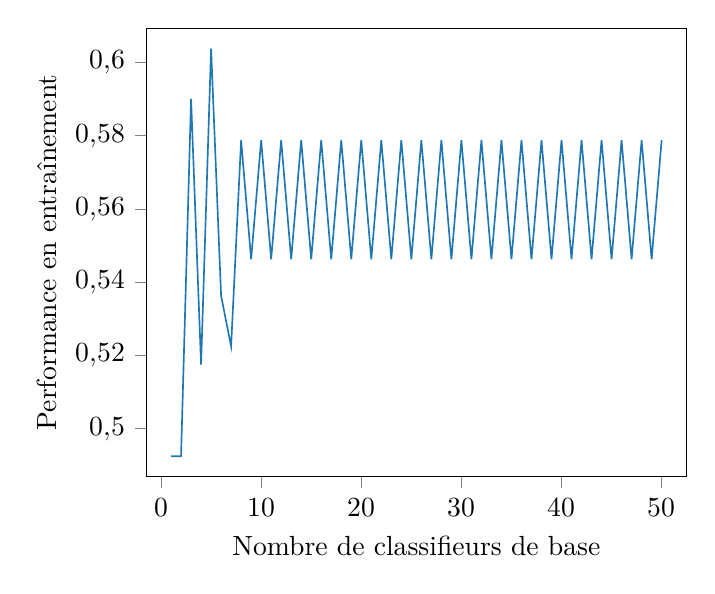
\begin{tikzpicture}

\definecolor{color0}{rgb}{0.12156862745098,0.466666666666667,0.705882352941177}

\begin{axis}[
tick align=outside,
tick pos=left,
x grid style={white!69.01960784313725!black},
xlabel={Nombre de classifieurs de base},
xmin=-1.45, xmax=52.45,
y grid style={white!69.01960784313725!black},
ylabel={Performance en entraînement},
ymin=0.4869375, ymax=0.6093125,
/pgf/number format/.cd,
use comma,
]
\addplot [semithick, color0, forget plot]
table [row sep=\\]{%
1	0.4925 \\
2	0.4925 \\
3	0.59 \\
4	0.5175 \\
5	0.60375 \\
6	0.53625 \\
7	0.5225 \\
8	0.57875 \\
9	0.54625 \\
10	0.57875 \\
11	0.54625 \\
12	0.57875 \\
13	0.54625 \\
14	0.57875 \\
15	0.54625 \\
16	0.57875 \\
17	0.54625 \\
18	0.57875 \\
19	0.54625 \\
20	0.57875 \\
21	0.54625 \\
22	0.57875 \\
23	0.54625 \\
24	0.57875 \\
25	0.54625 \\
26	0.57875 \\
27	0.54625 \\
28	0.57875 \\
29	0.54625 \\
30	0.57875 \\
31	0.54625 \\
32	0.57875 \\
33	0.54625 \\
34	0.57875 \\
35	0.54625 \\
36	0.57875 \\
37	0.54625 \\
38	0.57875 \\
39	0.54625 \\
40	0.57875 \\
41	0.54625 \\
42	0.57875 \\
43	0.54625 \\
44	0.57875 \\
45	0.54625 \\
46	0.57875 \\
47	0.54625 \\
48	0.57875 \\
49	0.54625 \\
50	0.57875 \\
};
\end{axis}

\end{tikzpicture}
	\caption{Performance en entraînement avec AdaBoost avec des souches de décision}
	\label{fig:adaboost_train_scores_with_decision_stumps}
\end{figure}
\begin{figure}
	\centering
	% This file was created by matplotlib2tikz v0.6.18.
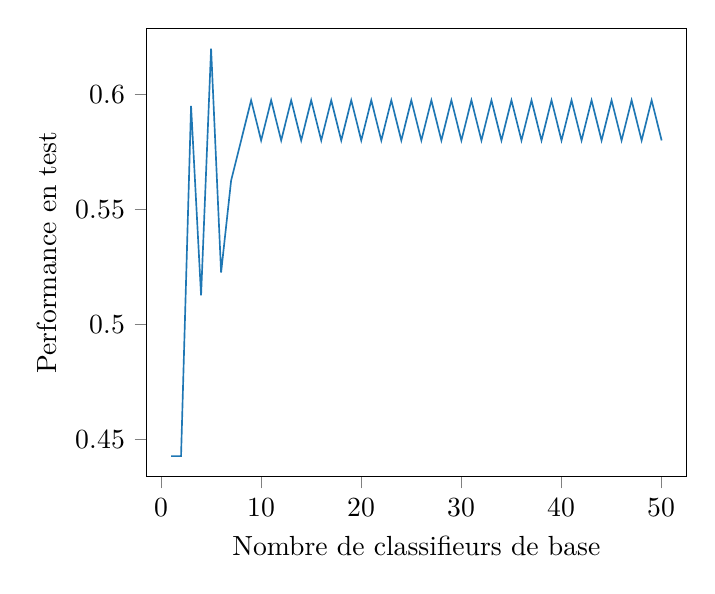
\begin{tikzpicture}

\definecolor{color0}{rgb}{0.12156862745098,0.466666666666667,0.705882352941177}

\begin{axis}[
tick align=outside,
tick pos=left,
x grid style={white!69.01960784313725!black},
xlabel={Nombre de classifieurs de base},
xmin=-1.45, xmax=52.45,
y grid style={white!69.01960784313725!black},
ylabel={Performance en test},
ymin=0.433625, ymax=0.628875
]
\addplot [semithick, color0, forget plot]
table [row sep=\\]{%
1	0.4425 \\
2	0.4425 \\
3	0.595 \\
4	0.5125 \\
5	0.62 \\
6	0.5225 \\
7	0.5625 \\
8	0.58 \\
9	0.5975 \\
10	0.58 \\
11	0.5975 \\
12	0.58 \\
13	0.5975 \\
14	0.58 \\
15	0.5975 \\
16	0.58 \\
17	0.5975 \\
18	0.58 \\
19	0.5975 \\
20	0.58 \\
21	0.5975 \\
22	0.58 \\
23	0.5975 \\
24	0.58 \\
25	0.5975 \\
26	0.58 \\
27	0.5975 \\
28	0.58 \\
29	0.5975 \\
30	0.58 \\
31	0.5975 \\
32	0.58 \\
33	0.5975 \\
34	0.58 \\
35	0.5975 \\
36	0.58 \\
37	0.5975 \\
38	0.58 \\
39	0.5975 \\
40	0.58 \\
41	0.5975 \\
42	0.58 \\
43	0.5975 \\
44	0.58 \\
45	0.5975 \\
46	0.58 \\
47	0.5975 \\
48	0.58 \\
49	0.5975 \\
50	0.58 \\
};
\end{axis}

\end{tikzpicture}
	\caption{Performance en test avec AdaBoost avec des souches de décision}
	\label{fig:adaboost_test_scores_with_decision_stumps}
\end{figure}
\directlua{dofile("decision_stump_figures.lua")}

La table~\ref{tab:adaboost_scores_with_decision_trees} donne les performances obtenues en utilisant des arbres de décision à trois niveaux comme classifieur de base.
\begin{table}
	\centering
	\caption{Performance en entraînement et en test avec AdaBoost avec des arbres de décision à trois niveaux}
	\begin{tabular}{S S S S S S}
		\toprule
			{\textbf{Estimateurs}}
			& {Entraînement}
			& {Test}
			& {\textbf{Estimateurs}}
			& {Entraînement}
			& {Test} \\
		\midrule
			1 & 0.80125 & 0.7525 & 26 & 0.85 & 0.8025 \\
			2 & 0.6975 & 0.66 & 27 & 0.8825 & 0.8275 \\
			3 & 0.7825 & 0.7425 & 28 & 0.88375 & 0.845 \\
			4 & 0.71625 & 0.69 & 29 & 0.895 & 0.87 \\
			5 & 0.69 & 0.6625 & 30 & 0.8975 & 0.865 \\
			6 & 0.63375 & 0.67 & 31 & 0.915 & 0.87 \\
			7 & 0.76375 & 0.775 & 32 & 0.91875 & 0.875 \\
			8 & 0.73125 & 0.7525 & 33 & 0.91875 & 0.8725 \\
			9 & 0.77875 & 0.7925 & 34 & 0.91 & 0.8775 \\
			10 & 0.76 & 0.765 & 35 & 0.9325 & 0.9 \\
			11 & 0.775 & 0.7925 & 36 & 0.9325 & 0.895 \\
			12 & 0.79 & 0.785 & 37 & 0.92125 & 0.8875 \\
			13 & 0.82 & 0.7975 & 38 & 0.91875 & 0.8825 \\
			14 & 0.88375 & 0.855 & 39 & 0.92625 & 0.88 \\
			15 & 0.87 & 0.8275 & 40 & 0.92375 & 0.8825 \\
			16 & 0.8825 & 0.8325 & 41 & 0.91125 & 0.885 \\
			17 & 0.84875 & 0.8275 & 42 & 0.93875 & 0.8975 \\
			18 & 0.87 & 0.83 & 43 & 0.93625 & 0.895 \\
			19 & 0.9025 & 0.845 & 44 & 0.9025 & 0.8825 \\
			20 & 0.905 & 0.86 & 45 & 0.8975 & 0.8725 \\
			21 & 0.88 & 0.85 & 46 & 0.89125 & 0.885 \\
			22 & 0.86 & 0.8325 & 47 & 0.8925 & 0.88 \\
			23 & 0.85375 & 0.8075 & 48 & 0.90125 & 0.875 \\
			24 & 0.86125 & 0.81 & 49 & 0.915 & 0.89 \\
			25 & 0.87625 & 0.8375 & 50 & 0.905 & 0.885 \\
		\bottomrule
	\end{tabular}
	\label{tab:adaboost_scores_with_decision_trees}
\end{table}
\begin{figure}
	\centering
	% This file was created by matplotlib2tikz v0.6.18.
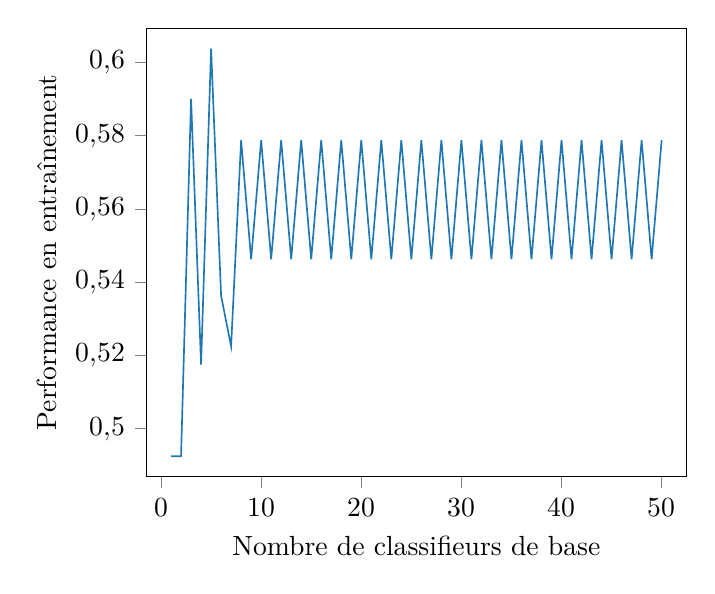
\begin{tikzpicture}

\definecolor{color0}{rgb}{0.12156862745098,0.466666666666667,0.705882352941177}

\begin{axis}[
tick align=outside,
tick pos=left,
x grid style={white!69.01960784313725!black},
xlabel={Nombre de classifieurs de base},
xmin=-1.45, xmax=52.45,
y grid style={white!69.01960784313725!black},
ylabel={Performance en entraînement},
ymin=0.4869375, ymax=0.6093125,
/pgf/number format/.cd,
use comma,
]
\addplot [semithick, color0, forget plot]
table [row sep=\\]{%
1	0.4925 \\
2	0.4925 \\
3	0.59 \\
4	0.5175 \\
5	0.60375 \\
6	0.53625 \\
7	0.5225 \\
8	0.57875 \\
9	0.54625 \\
10	0.57875 \\
11	0.54625 \\
12	0.57875 \\
13	0.54625 \\
14	0.57875 \\
15	0.54625 \\
16	0.57875 \\
17	0.54625 \\
18	0.57875 \\
19	0.54625 \\
20	0.57875 \\
21	0.54625 \\
22	0.57875 \\
23	0.54625 \\
24	0.57875 \\
25	0.54625 \\
26	0.57875 \\
27	0.54625 \\
28	0.57875 \\
29	0.54625 \\
30	0.57875 \\
31	0.54625 \\
32	0.57875 \\
33	0.54625 \\
34	0.57875 \\
35	0.54625 \\
36	0.57875 \\
37	0.54625 \\
38	0.57875 \\
39	0.54625 \\
40	0.57875 \\
41	0.54625 \\
42	0.57875 \\
43	0.54625 \\
44	0.57875 \\
45	0.54625 \\
46	0.57875 \\
47	0.54625 \\
48	0.57875 \\
49	0.54625 \\
50	0.57875 \\
};
\end{axis}

\end{tikzpicture}
	\caption{Performance en entraînement avec AdaBoost avec des arbres de décision à trois niveaux}
	\label{fig:adaboost_train_scores_with_decision_trees}
\end{figure}
\begin{figure}
	\centering
	% This file was created by matplotlib2tikz v0.6.18.
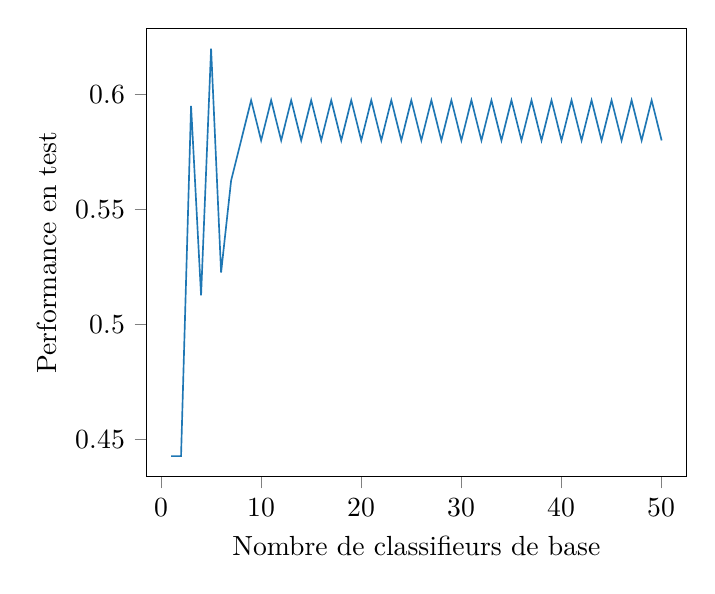
\begin{tikzpicture}

\definecolor{color0}{rgb}{0.12156862745098,0.466666666666667,0.705882352941177}

\begin{axis}[
tick align=outside,
tick pos=left,
x grid style={white!69.01960784313725!black},
xlabel={Nombre de classifieurs de base},
xmin=-1.45, xmax=52.45,
y grid style={white!69.01960784313725!black},
ylabel={Performance en test},
ymin=0.433625, ymax=0.628875
]
\addplot [semithick, color0, forget plot]
table [row sep=\\]{%
1	0.4425 \\
2	0.4425 \\
3	0.595 \\
4	0.5125 \\
5	0.62 \\
6	0.5225 \\
7	0.5625 \\
8	0.58 \\
9	0.5975 \\
10	0.58 \\
11	0.5975 \\
12	0.58 \\
13	0.5975 \\
14	0.58 \\
15	0.5975 \\
16	0.58 \\
17	0.5975 \\
18	0.58 \\
19	0.5975 \\
20	0.58 \\
21	0.5975 \\
22	0.58 \\
23	0.5975 \\
24	0.58 \\
25	0.5975 \\
26	0.58 \\
27	0.5975 \\
28	0.58 \\
29	0.5975 \\
30	0.58 \\
31	0.5975 \\
32	0.58 \\
33	0.5975 \\
34	0.58 \\
35	0.5975 \\
36	0.58 \\
37	0.5975 \\
38	0.58 \\
39	0.5975 \\
40	0.58 \\
41	0.5975 \\
42	0.58 \\
43	0.5975 \\
44	0.58 \\
45	0.5975 \\
46	0.58 \\
47	0.5975 \\
48	0.58 \\
49	0.5975 \\
50	0.58 \\
};
\end{axis}

\end{tikzpicture}
	\caption{Performance en test avec AdaBoost avec des arbres de décision à trois niveaux}
	\label{fig:adaboost_test_scores_with_decision_trees}
\end{figure}
\directlua{dofile("decision_tree_figures.lua")}

\section{Réduction de dimensionnalité}

\end{document}
